\documentclass{beamer}
\usetheme[numbering=progressbar]{misp}

\usepackage[utf8]{inputenc}
\usepackage{booktabs}
\usepackage{array}
\usepackage{listings}
\usetikzlibrary{positioning,arrows.meta}

\lstdefinestyle{modulecode}{
    basicstyle=\ttfamily\scriptsize,
    backgroundcolor=\color{mispBlue!5!white},
    frame=single,
    rulecolor=\color{mispBlue!30!white},
    breaklines=true,
    columns=fullflexible,
    keepspaces=true,
    showstringspaces=false,
    numbers=none,
    aboveskip=.6em,
    belowskip=.6em
}
\lstdefinelanguage{json}{
    morestring=[b]",
    keywords={true,false,null},
    sensitive=true
}
\lstset{style=modulecode}
\newcolumntype{P}[1]{>{\raggedright\arraybackslash}p{#1}}
\newcommand{\code}[1]{\texttt{\detokenize{#1}}}
\newcommand{\sources}[1]{\par\vfill{\tiny\color{mispTeal}#1\par}}

\title{MISP modules}
\subtitle{Enrichment, data exchange and workflow actions}
\author{\small CIRCL / MISP Project}
\institute{\url{https://www.misp-project.org/}}
\date{Reference snapshot: 29 October 2026}

\begin{document}
% Included by slide.tex. Source audit and runnable examples: README.md.
\begin{frame}[t,plain]
    \titlepage
\end{frame}

\begin{frame}{What you will be able to do}
    \begin{enumerate}
        \item Select and discover modules for an analyst's task.
        \item Connect MISP to a working module service.
        \item Operate configuration, caching and query diagnostics.
        \item Generate exports and distinguish them from workflow actions.
        \item Use the standalone website and develop a local module.
    \end{enumerate}
    \begin{block}{Hands-on route}
        The accompanying lab uses synthetic data, local processing and an
        explicit dry run. No provider account or running MISP instance is needed.
    \end{block}
    \note{Use this as a 60--90 minute session, extending the optional development lab.
    Ask which roles are present: analyst, platform operator, integration developer.
    The README provides shorter teaching routes and expected exercise outcomes.}
\end{frame}

\begin{frame}{A dated snapshot, not a promise about every install}
    \begin{itemize}
        \item Reviewed against upstream \code{main}, commit \code{3a903305cf37},
        on 29 October 2026.
        \item Package metadata declares version \code{3.1.1}.
        Features on this branch can postdate a published package.
        \item Source inventory: \textbf{270 candidate module files} across four families.
        \item Installed dependencies, credentials and service reachability determine
        which integrations can actually run.
    \end{itemize}
    \begin{block}{Inspect the running service}
        Check \code{/version}, \code{/modules} and \code{/openapi.json}.
        A source file count is not the number of operational integrations.
    \end{block}
    \sources{Pinned source links and the inventory method are in this deck's README.}
    \note{The count excludes \_\_init\_\_.py and underscore-prefixed files.
    Do not present 3.1.1 as guaranteeing every feature in this training.
    Recheck the revision before teaching a later release.}
\end{frame}

\begin{frame}{Four families, different contracts}
    \small
    \begin{tabular}{@{}P{2cm}P{2.6cm}rP{4.6cm}@{}}
        \toprule
        Family & Directory & Files & Purpose \\
        \midrule
        Expansion & \code{expansion} & 203 &
        Enrich an observable; some modules also support hover. \\
        Import & \code{import_mod} & 22 &
        Parse uploaded data or retrieve a report into MISP results. \\
        Export & \code{export_mod} & 32 &
        Transform supplied MISP data into a downloadable format. \\
        Action & \code{action_mod} & 13 &
        Run an operation from a workflow, such as a notification or publication. \\
        \bottomrule
    \end{tabular}
    \medskip
    Directory names are loader families. Metadata uses
    \code{expansion}/\code{hover}, \code{import}, \code{export} and \code{action}.
    \note{These are the four ModuleType values in misp-modules, not every integration
    family recognized by MISP core. Cortex and other core integrations are separate.
    Hover is a capability of expansion modules, not a fifth directory.}
\end{frame}

\begin{frame}{One service, several clients}
    \centering
    \begin{tikzpicture}[
        box/.style={draw=mispTeal,rounded corners,align=center,
                    fill=mispBlue!5!white,font=\small,minimum height=1cm},
        flow/.style={-{Stealth},thick,draw=mispTeal}]
        \node[box,text width=2.6cm] (misp) at (0,2) {MISP\\analyst UI / workflows};
        \node[box,text width=2.6cm] (web) at (0,.4) {Standalone website};
        \node[box,text width=2.6cm] (api) at (0,-1.2) {Scripts / API clients};
        \node[box,text width=3cm,minimum height=3.8cm] (service) at (4,.4)
            {\textbf{misp-modules}\\[.5em]Discovery\\and dispatch\\Local defaults\\Optional cache\\Statistics};
        \node[box,text width=2.4cm] (local) at (8,1.5) {Local parsers\\and datasets};
        \node[box,text width=2.4cm] (remote) at (8,-.6) {Provider APIs\\or action targets};
        \draw[flow] (misp.east) -- (service.west);
        \draw[flow] (web.east) -- (service.west);
        \node[font=\scriptsize,text=mispTeal] at (4,2.8) {HTTP / JSON API};
        \draw[flow] (api.east) -- (service.west);
        \draw[flow] (service.east) -- (local.west);
        \draw[flow] (service.east) -- (remote.west);
    \end{tikzpicture}
    \sources{The Python service can run without a MISP server. The website is a separate application.}
    \note{The service can be co-located with MISP or run elsewhere.
    Distinguish MISP's event database, the module process, and the website's own
    database/session history. They are not a shared persistence layer.
    Some operations are local; many enrichments contact third parties.}
\end{frame}

\section{Use and understand modules}

\begin{frame}{Choose a module by the question you need to answer}
    \small
    \begin{tabular}{P{3.9cm}P{6.5cm}}
        \toprule
        Analyst question & Examples in the current source \\
        \midrule
        What does this URL contain? & \code{extract_url_components}: local structured parsing. \\
        What infrastructure is related? & \code{dns}, \code{reversedns}, \code{circl_passivedns}: different DNS evidence. \\
        Is this observable known or noisy? & \code{hygiene}, \code{hashlookup}, \code{greynoise}. \\
        What vulnerability context exists? & \code{cve}, \code{gcve_cpe}, \code{rapid7_attackerkb}. \\
        What does analysis tooling know? & \code{mwdb_query}, \code{assemblyline_query}, sandbox query/submit integrations. \\
        \bottomrule
    \end{tabular}
    \medskip
    Read the module's input types, configuration, dependencies and side effects.
    A lookup and a submission are different operational choices.
    \note{Examples are representative, not an endorsement or a complete catalog.
    Hygiene adds local warninglist context; a match is not proof of benignness.
    GCVE CPE matches a catalog record and does not establish that a product is vulnerable.
    Provider coverage depends on API version, account entitlement and quotas.}
\end{frame}

\begin{frame}[fragile]{Discover what is really loaded}
\begin{lstlisting}[language=bash]
curl --fail --silent --show-error \
  http://127.0.0.1:6666/modules |
  jq '.[] | {name, type, mispattributes, meta}'
\end{lstlisting}
    \begin{itemize}
        \item \code{name}: API identifier, usually the Python filename.
        \item \code{meta.name}: human-readable display name, when supplied.
        \item \code{mispattributes}: input/output capabilities and format.
        \item \code{meta.config}: expected settings, not configured secret values.
        \item \code{meta.module-type}: capabilities used by MISP.
    \end{itemize}
    \note{A missing optional library can cause the loader to skip a module.
    The metadata requirements field is descriptive; it does not install libraries.
    Restart after code changes; module loading and OpenAPI generation happen at startup.
    Teach participants to select by API identifier rather than display name.}
\end{frame}

\begin{frame}[fragile]{Two expansion formats still coexist}
    \begin{columns}[T]
        \column{.48\textwidth}
        \textbf{Simplified / legacy}
\begin{lstlisting}[language=json]
{"module": "training_uppercase",
 "text": "misp training"}

{"results": [
  {"types": ["text"],
   "values": ["LOCAL: MISP TRAINING"]}
]}
\end{lstlisting}
        \column{.48\textwidth}
        \textbf{MISP standard}
\begin{lstlisting}[language=json]
{"module": "...",
 "attribute": {
   "type": "url",
   "value": "...",
   "uuid": "..."
 }}

{"results": {
  "Attribute": [], "Object": []
}}
\end{lstlisting}
    \end{columns}
    \small
    The module's introspection selects the contract.
    \code{format: misp_standard} enables structured results and references.
    \note{The ellipses on the right describe the shape, not a runnable payload.
    The next slide supplies a complete example. Do not send one universal request
    shape to every module. Some structured modules also return Tag data.
    The left example uses the lab prefix defaults and the legacy result format.}
\end{frame}

\begin{frame}[fragile]{A complete local enrichment request}
    \small
    Save or use the included \code{examples/url-request.json}:
    \lstinputlisting[language=json]{examples/url-request.json}
\begin{lstlisting}[language=bash]
curl --fail --silent --show-error \
  http://127.0.0.1:6666/query \
  -H 'Content-Type: application/json' \
  --data @examples/url-request.json
\end{lstlisting}
    \note{Run from this deck's directory. This module parses the URL locally:
    it does not fetch portal.example.org. The UUID is a synthetic source attribute.
    Show the complete response, then find results.Object and the url object.
    The lab verifies the domain, host, resource path and source reference.}
\end{frame}

\begin{frame}{Read the result as evidence}
    \begin{itemize}
        \item URL parsing produces a \code{url} object, its component attributes,
        and a reference to the source attribute.
        \item Current DNS enrichment can express a \code{dns-record} object and
        related records, rather than flattening a lookup to one IP.
        \item Keep source identifiers and object references when pivoting.
        \item Review provenance, time, relevance and sharing constraints before
        adding or using results.
    \end{itemize}
    \begin{block}{Enrichment is not a detection verdict}
        Context, reputation, warninglist matches and generated rules still need
        an analyst's interpretation.
    \end{block}
    \note{Avoid the old hardcoded DNS answer or a claim that all domains map to one
    address. An observed DNS answer is time-bound; passive DNS and active resolution
    answer different questions. Review detection flags before promoting enrichment
    into a downstream control.}
\end{frame}

\begin{frame}{Connect MISP: service discovery and user access}
    \small
    In \textbf{Administration $\rightarrow$ Server Settings \& Maintenance
    $\rightarrow$ Plugin settings}:
    \begin{enumerate}
        \item Configure the relevant service family: \code{Enrichment},
        \code{Import}, \code{Export} or \code{Action}.
        \item Set its \code{services_enable}, \code{services_url} and
        \code{services_port} settings.
        \item Reload settings, enable the desired module and set its credentials.
        \item Check organisation restrictions and supported input types.
    \end{enumerate}
    \begin{block}{Example}
        \code{Plugin.Enrichment_services_enable}\\
        Enable the enrichment family, then enable/configure its individual modules.
    \end{block}
    \sources{Verify connectivity from the MISP host/container; its localhost may not be the module server.}
    \note{Enabling Enrichment does not enable Import, Export or Action.
    The current MISP Module model checks each family's enable switch and builds its URL.
    Action module parameters and workflow behavior are module-specific.
    Distinguish service startup, discovery, MISP enablement and user permissions:
    each is a separate checkpoint.}
\end{frame}

\section{Deploy and operate the service}

\begin{frame}{Choose the dependency footprint}
    \small
    \begin{tabular}{P{2.2cm}P{3cm}P{4.8cm}}
        \toprule
        Install & Python command & What to expect \\
        \midrule
        Base & \code{pip install .} &
        Core service, workflow support and modules whose imports are satisfied. \\
        Common extras & \code{pip install '.[minimal]'} &
        A broader set of Python dependencies, intended without extra system packages. \\
        Broad extras & \code{pip install '.[all]'} &
        Wider coverage; some native tools/libraries are also required. \\
        \bottomrule
    \end{tabular}
    \medskip
    The snapshot requires \textbf{Python 3.10 or newer, below 4.0}.
    The lab uses Python 3.12 and the base installation.
    \note{Run these commands from a source checkout inside a virtual environment.
    For a published package the equivalents are misp-modules, misp-modules[minimal],
    and misp-modules[all]. Shell-quote extras.
    Native examples include Poppler, zbar and Tesseract. Installing all extras
    does not create provider accounts, API entitlements or valid credentials.
    A missing-yara warning is a heuristic for reduced dependencies, not proof
    that every other module failed.}
\end{frame}

\begin{frame}[fragile]{Use a virtual environment and a supervised process}
\begin{lstlisting}[language=bash]
git clone https://github.com/MISP/misp-modules.git
cd misp-modules
python3 -m venv .venv
. .venv/bin/activate
python -m pip install .
misp-modules -l 127.0.0.1 -p 6666
\end{lstlisting}
    \begin{itemize}
        \item Pin a reviewed revision for a reproducible workshop.
        \item For development, use an editable installation or Poetry.
        \item In production, use a service manager with the actual venv executable
        and service account.
    \end{itemize}
    \sources{No global sudo pip installation or rc.local startup is needed. See the README for the pinned lab setup.}
    \note{The slide shows the generic source workflow; the README adds the exact
    reviewed commit before installation. systemd does not source a user's shell
    profile or venv activation. Retain existing startup flags in service overrides.
    Remote/container deployments need an address reachable from MISP and an appropriate
    access boundary; do not expose the raw service to the Internet.}
\end{frame}

\begin{frame}{The service API is discoverable}
    \small
    \begin{tabular}{P{3.1cm}P{7.1cm}}
        \toprule
        Endpoint & What it tells you \\
        \midrule
        \code{GET /healthcheck} & The HTTP service is responding. \\
        \code{GET /version} & Installed package version. \\
        \code{GET /modules} & Loaded module metadata and capabilities. \\
        \code{GET /openapi.json} & Startup-generated API specification. \\
        \code{GET /openapi} & Interactive Swagger UI using that specification. \\
        \code{POST /query} & Dispatch a request to one selected module. \\
        \code{GET /statistics} & Query counts, outcomes, latency and optional cache metrics. \\
        \bottomrule
    \end{tabular}
    \medskip
    A healthy service does not prove that a provider query will succeed.
    \note{Restart after adding/removing modules to refresh discovery and OpenAPI.
    Swagger UI assets are referenced from a CDN; the JSON specification remains
    useful without those browser assets. The service API is independent of the
    standalone website and its login/database.
    Core requests can succeed at HTTP level while returning a module error envelope.}
\end{frame}

\begin{frame}{Configure the right layer}
    \begin{itemize}
        \item \textbf{MISP settings}: enablement, organisation restrictions and
        configuration sent in a query's \code{config}.
        \item \textbf{Module-server defaults}: optional
        \code{--module-config} JSON for credentials, URLs and other settings.
        \item \textbf{Service environment}: used by integrations that explicitly
        read environment variables, including some publication actions.
        \item \textbf{Website settings}: a separate application and stored module
        settings; not the MISP database.
    \end{itemize}
    \note{Do not assume that a setting in MISP's UI becomes an environment variable
    in a systemd service. Conversely, a module server's local defaults do not enable
    that module in MISP. Action modules may use params and environment variables;
    the generic config mechanism does not replace their documented contracts.}
\end{frame}

\begin{frame}[fragile]{Local defaults: explicit precedence}
    \lstinputlisting[language=json]{examples/module-defaults.json}
    \small
    Start with \code{--module-config examples/module-defaults.json}.
    \begin{itemize}
        \item Missing settings use defaults; explicit API values win.
        \item Empty strings/null use defaults only for named
        \code{fallback_when_empty} keys.
        \item Read once at startup; restart after edits or credential rotation.
    \end{itemize}
    \note{The file contains synthetic prefix text, not credentials.
    The lab verifies missing config, a nonempty override and empty/null fallback.
    False, zero, empty lists/objects are explicit values, not empty-string fallbacks.
    No recursive merging or environment-variable interpolation is performed.
    Any caller reaching the service can use its local defaults: separate trust
    boundaries may need separate module services.}
\end{frame}

\begin{frame}{Optional caching: choose read-only expansions}
    \begin{itemize}
        \item Enable with \code{--cache-config}; disabled by default.
        \item Opt in each expansion module, with a TTL, entry limit and response-byte limit.
        \item Match the \textbf{whole effective request}, after local defaults:
        UUIDs, context, credentials and timeout matter.
        \item Identical concurrent requests can share one execution.
        \item Cache entries and counters are process-local and reset on restart.
    \end{itemize}
    \begin{block}{Choose by behavior, not just family}
        Some expansion modules submit data or cause side effects.
        Caching one can suppress a repeated operation.
    \end{block}
    \note{No Redis or external cache is required by the current optional cache.
    Import/export/action modules cannot be configured as loaded cached modules.
    Errors and late results are not retained; empty successful results can be.
    Hits do not extend expiry. Different attribute UUIDs deliberately do not share
    the same complete response. This is not a provider-wide rate limiter.}
\end{frame}

\begin{frame}[fragile]{Observe queries, failures and cache savings}
\begin{lstlisting}[language=bash]
curl --fail --silent --show-error \
  http://127.0.0.1:6666/statistics | jq .
\end{lstlisting}
    \begin{itemize}
        \item Per-module and aggregate counts include loaded, unused modules.
        \item Distinguish module errors, exceptions and timeouts.
        \item Compare success/error rates, latency and in-flight requests.
        \item Optional cache metrics include hits, misses and coalesced queries.
        \item Query counts measure service requests, not provider HTTP calls.
    \end{itemize}
    \note{Statistics are in memory per process and reset on restart.
    HTTP 200 with nonempty error/errors is a module failure, even with partial results.
    MISP supplies its own request timeout; direct service calls default to 300 seconds
    in this snapshot. A response timeout does not guarantee that the worker or remote
    operation stopped. Configure bounded provider-client timeouts in module code.}
\end{frame}


\begin{frame}{Operate the service within its trust boundary}
    \begin{itemize}
        \item Keep the API reachable only by intended clients; it has no built-in
        authentication layer in the reviewed dispatcher.
        \item Review which modules contact providers or submit samples.
        \item Keep local credentials outside the checkout and readable only by
        the service account.
        \item Use normal debug logs first.
        \code{--debug-extended} logs outbound \code{requests} exchanges,
        including credentials and full payloads.
    \end{itemize}
    \note{This is an operational consequence of the features, not a claim that every
    module has identical secret handling. Extended tracing is unredacted and only
    covers requests and SDKs using its standard adapter, not every HTTP library.
    Direct Python handler calls bypass dispatcher defaults, cache and
    statistics. A website admin login does not add authentication to the raw API.}
\end{frame}

\begin{frame}{Troubleshoot the failing layer}
    \small
    \begin{tabular}{P{3.2cm}P{7cm}}
        \toprule
        Symptom & First checks \\
        \midrule
        Cannot reach service & Process, listen address, container network, host/port. \\
        Module absent & Correct venv/package, optional dependencies, loader logs, restart. \\
        Present, absent in MISP & Correct family settings, metadata type, reload settings. \\
        Visible, unavailable to user & Module enablement, organisation restriction, supported input. \\
        HTTP 200, failed query & Inspect \code{error}/\code{errors}; config, quotas, provider response. \\
        Unexpected stale result & Effective request, TTL, correct process and cache configuration. \\
        \bottomrule
    \end{tabular}
    \note{Work from service health to discovery to module execution to UI.
    Run connectivity checks inside the MISP host/container, not only on the module
    server. Syntax errors can prevent startup; missing optional imports are often
    skipped. A local source edit is ineffective if the running service uses a
    different installed package or never restarted.}
\end{frame}

\section{Import, export and act}

\begin{frame}{Import: turn external material into MISP data}
    \begin{itemize}
        \item Import sources vary: file upload, pasted text, or remote report retrieval.
        \item Check \code{inputSource}, \code{userConfig} and module settings.
        \item File-oriented API requests commonly carry base64 \code{data}.
        \item Review returned attributes, objects and references before ingestion.
        \item Examples include email, sandbox reports, PCAP and TAXII integrations.
    \end{itemize}
    \begin{block}{Use the module's actual contract}
        A remote-report importer may need configuration instead of an uploaded file.
        File and report inputs are not interchangeable.
    \end{block}
    \note{Do not treat the testimport teaching stub as a production CSV parser.
    The standalone website now supports active import modules, including upload/paste
    and remote-report forms. Uploaded inputs are not saved for replay there.
    Review per-module schemas and external effects before using real reports.}
\end{frame}

\begin{frame}{Export modules are an active part of the platform}
    \small
    \begin{tabular}{P{3.1cm}P{7.1cm}}
        \toprule
        Target & Examples / output \\
        \midrule
        Detection and SIEM & \code{zeek_intel_export}, \code{elastic_ecs_export},
        \code{splunk_export}, \code{wazuh_cdb_export}. \\
        Host investigation & \code{osqueryexport}: query pack by default, optional raw SQL. \\
        Network policy & PAN-OS, Junos, FortiOS, ASA, RouterOS, PF and nftables exporters. \\
        Data interchange & CSV and other module-specific formats. \\
        \bottomrule
    \end{tabular}
    \medskip
    Native MISP exports also remain useful. Choose by target format and supported
    data, not an old assumption that module exports will disappear.
    \note{The current source has 32 export module files.
    Event collections and object attributes are supported by several newer exporters;
    some exporters still require a single event. Check each module's contract.
    Network ACL fragments are vendor-specific: a generic rule is not portable
    across devices, and an exported file has not been activated.}
\end{frame}

\begin{frame}[fragile]{Lab: generate a Zeek Intel file}
    Use the included \code{examples/export-request.json}.
\begin{lstlisting}[language=bash]
curl --fail --silent --show-error \
  http://127.0.0.1:6666/query \
  -H 'Content-Type: application/json' \
  --data @examples/export-request.json > /tmp/zeek-response.json

python3 -c 'import base64,json; r=json.load(open("/tmp/zeek-response.json")); print(base64.b64decode(r["data"]).decode("ascii"))'
\end{lstlisting}
    \small
    Expected: \code{example.org} and \code{192.0.2.10}, with native Zeek types.
    The non-IDS attribute is excluded by default.
    \note{The response envelope's data is base64, not an event JSON document.
    In automation, check error/errors before decoding data.
    The functional lab verifies the \#fields header, Intel::DOMAIN/ADDR and non-IDS
    exclusion. No Zeek service is contacted or reloaded.
    Distribution, policy loading and operational detection checks remain separate.}
\end{frame}

\begin{frame}{Exporting a file and publishing an action differ}
    \small
    \begin{tabular}{P{2.5cm}P{4cm}P{3.5cm}}
        \toprule
        & Export & Workflow action \\
        \midrule
        Main result & A file or generated representation. & An operation and its status/result. \\
        Examples & Zeek feed, osquery pack, firewall fragment. & Notification, local pack write, SIEM/EDR publication. \\
        Credentials & Often unnecessary for local generation. & Often needed for the target; some support credential-free dry runs. \\
        Completion & Output generated. & Check acknowledgement, partial failures and activation requirements. \\
        \bottomrule
    \end{tabular}
    \note{Neither family is guaranteed side-effect-free: some exports contact services,
    and some expansions submit data. Classify actual behavior.
    An action can publish to an endpoint, or only write a local artifact.
    Do not equate a successful export, local publication, target acknowledgement
    and effective detection on endpoints.}
\end{frame}

\begin{frame}{Workflow actions connect intelligence to operations}
    \begin{itemize}
        \item Notifications: Slack, Matrix, IRC, Signal and Nextcloud Talk.
        \item Target publication: CrowdStrike IOC, SentinelOne IOC,
        QRadar reference sets and Wazuh CDB lists.
        \item Local artifact publication: \code{osquery_pack_publish}.
        \item Inspect action metadata: parameters, blocking behavior,
        filters and expected MISP-core format.
        \item Supply the intended data selection and explicit target scope.
    \end{itemize}
    \note{Action request parameters usually live in params, not the expansion config
    object. Individual actions can also require credentials in the service environment.
    Some actions do not support workflow filteredItems/matchingData; do not assume
    every action consumes an identical workflow payload.
    Blocking action failures can stop a workflow path; inspect its returned data
    and module-specific errors, including partial publication failures.}
\end{frame}

\begin{frame}[fragile]{Lab: plan an osquery publication}
    \lstinputlisting[language=json]{examples/action-request.json}
    \small
    Expected: \code{data.status = planned}, a pack and provenance.
    This dry run writes no pack and executes no endpoint queries.
    \note{The included API verification asserts planned rather than published.
    Real local publication needs OSQUERY\_PACK\_DIRECTORY on the module server.
    Existing packs require explicit overwrite, which replaces the complete snapshot.
    The action does not implement a generic push API to an osquery agent:
    distribute/reference the pack and reload configuration separately.
    Other actions have different defaults; request dry\_run explicitly where supported.}
\end{frame}

\section{The standalone website}

\begin{frame}{An enrichment workspace without a MISP instance}
    \centering
    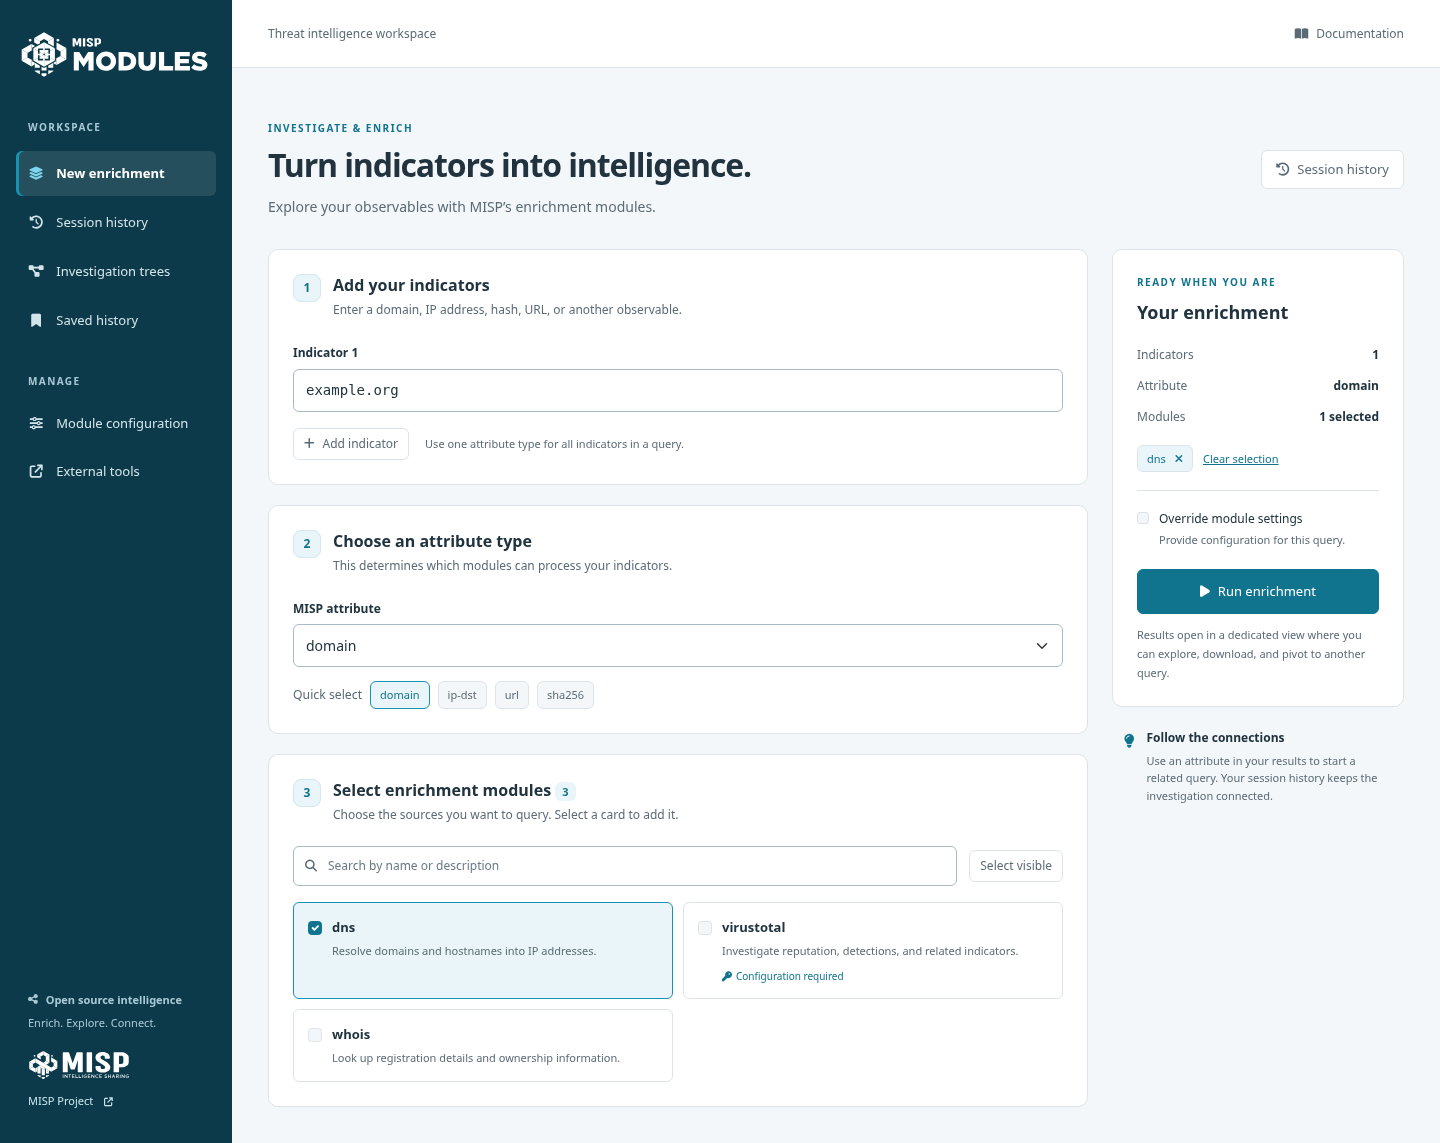
\includegraphics[width=\textwidth,height=.66\paperheight,keepaspectratio]{screenshots/current/workspace.png}
    \sources{Current upstream documentation screenshot; sample catalogue from browser fixtures.}
    \note{Choose the attribute type, compatible modules and indicators before submitting.
    Changing attribute type clears incompatible selections.
    Per-query overrides are separate from saved module settings.
    The website is a client of the same module service, not a MISP event database.
    This screenshot is upstream's illustrative browser-test capture, not a live provider test.}
\end{frame}

\begin{frame}{Structured results and investigation pivots}
    \begin{columns}[T]
        \column{.48\textwidth}
        \centering
        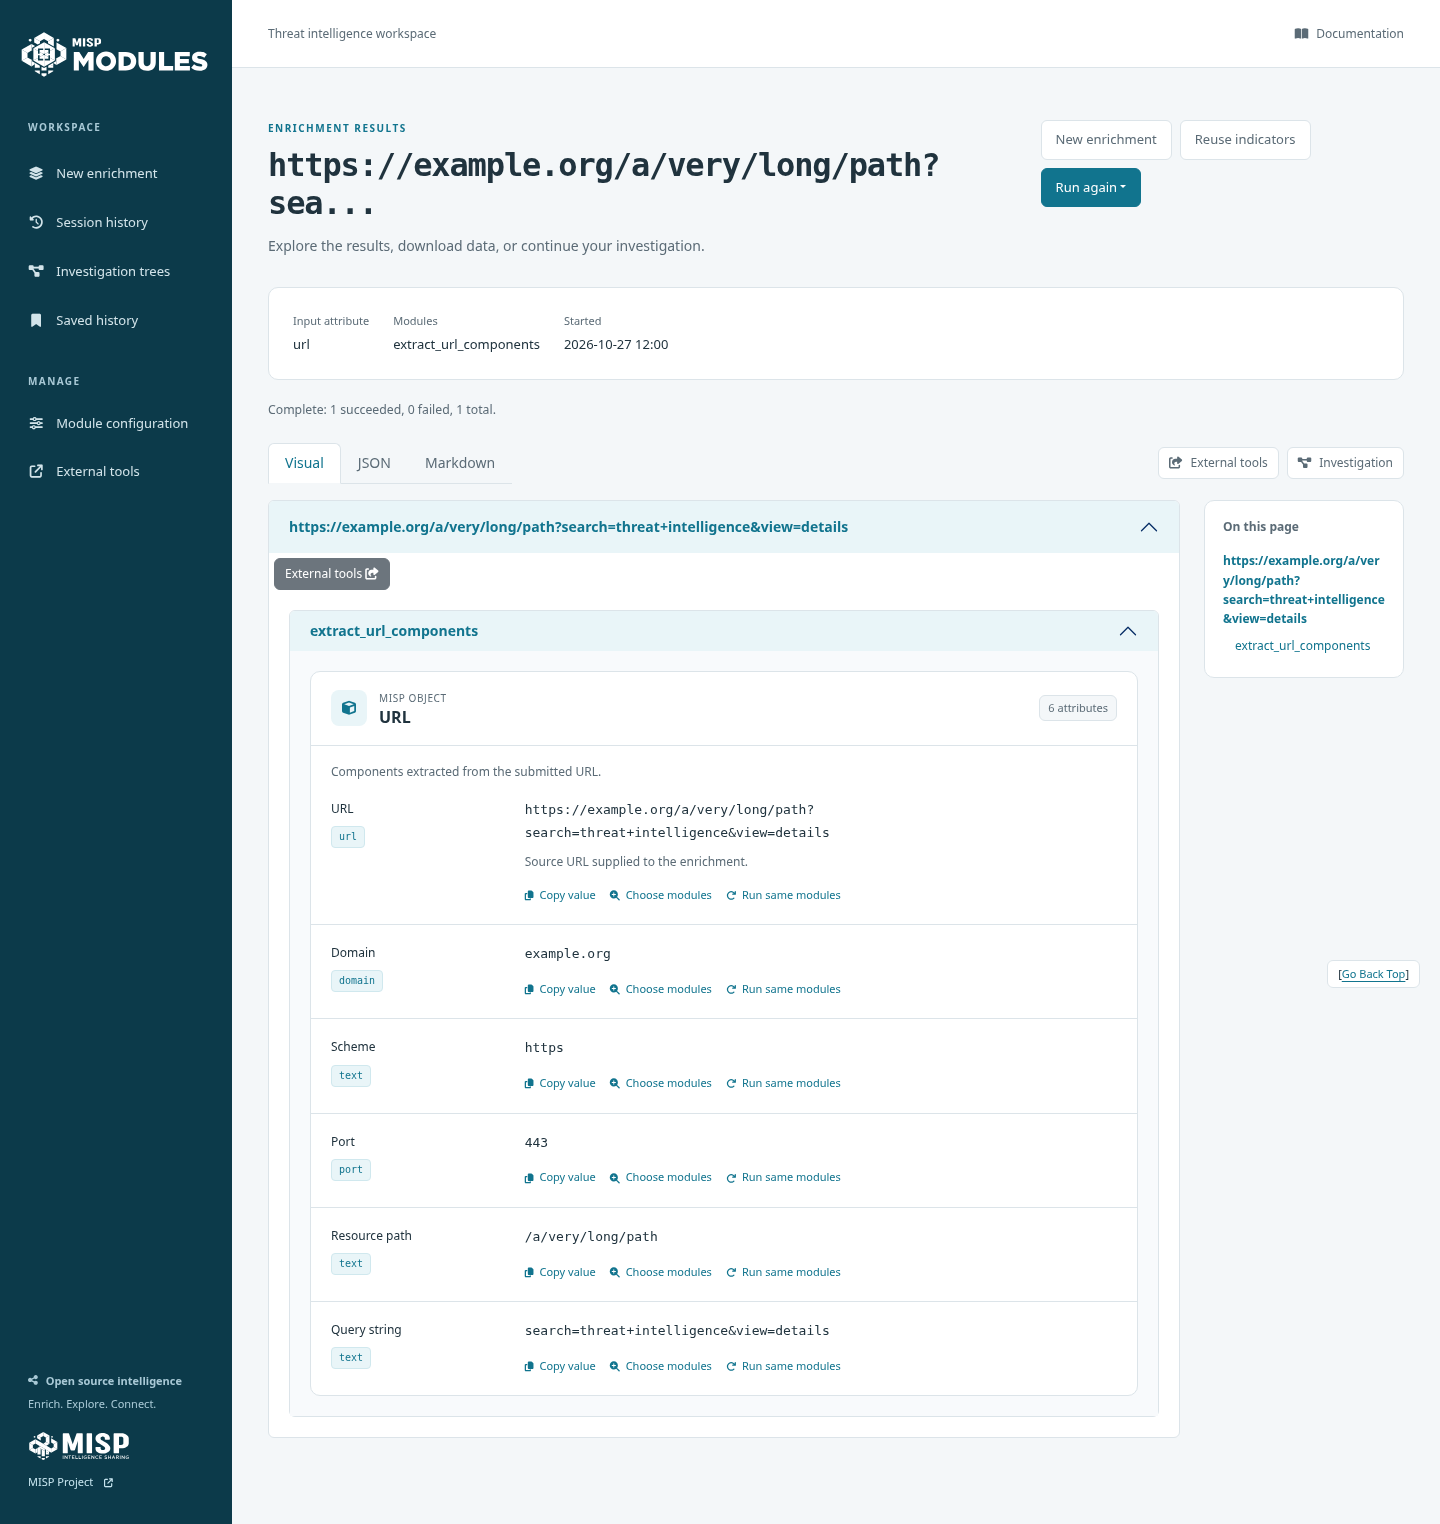
\includegraphics[width=\linewidth,height=.62\paperheight,keepaspectratio]{screenshots/current/results.png}
        \column{.48\textwidth}
        \begin{itemize}
            \item Separate object cards and flat attributes.
            \item Visual, JSON and Markdown views.
            \item Copy complete values or start a related enrichment.
            \item Download results and use configured external tools.
        \end{itemize}
    \end{columns}
    \sources{Source: website/doc/interface.md and \code{object_result_cards.png} at the reviewed revision.}
    \note{The old deck called external tools still in development.
    The current application implements configured external-tool flows; availability
    depends on configured destinations and their keys. A current migration repairs
    legacy external\_tools.api\_key schema state.
    Rendering and a copy action do not establish provider availability or publication success.}
\end{frame}

\begin{frame}{Import and export are website workflows too}
    \begin{itemize}
        \item \textbf{Import data}: choose an active module and provide a supported
        upload, paste or remote-report configuration.
        \item \textbf{Export data}: provide MISP JSON, or choose a CIRCL OSINT feed
        event, then configure an active exporter.
        \item Results, text previews, decoded downloads and history use the shared interface.
        \item With \code{ADMIN_PASSWORD} configured, exports and their saved results
        require an administrator login.
    \end{itemize}
    \note{The reviewed website bounds uploads to 20 MiB. It accepts several event
    envelope shapes but honors modules that require a single event.
    Feed access occurs on the website server, not in the browser.
    Uploaded import/export input is not retained for replay; provide it again on a new run.
    The raw service and website authentication boundaries are separate.}
\end{frame}

\begin{frame}{Keep the investigation path}
    \centering
    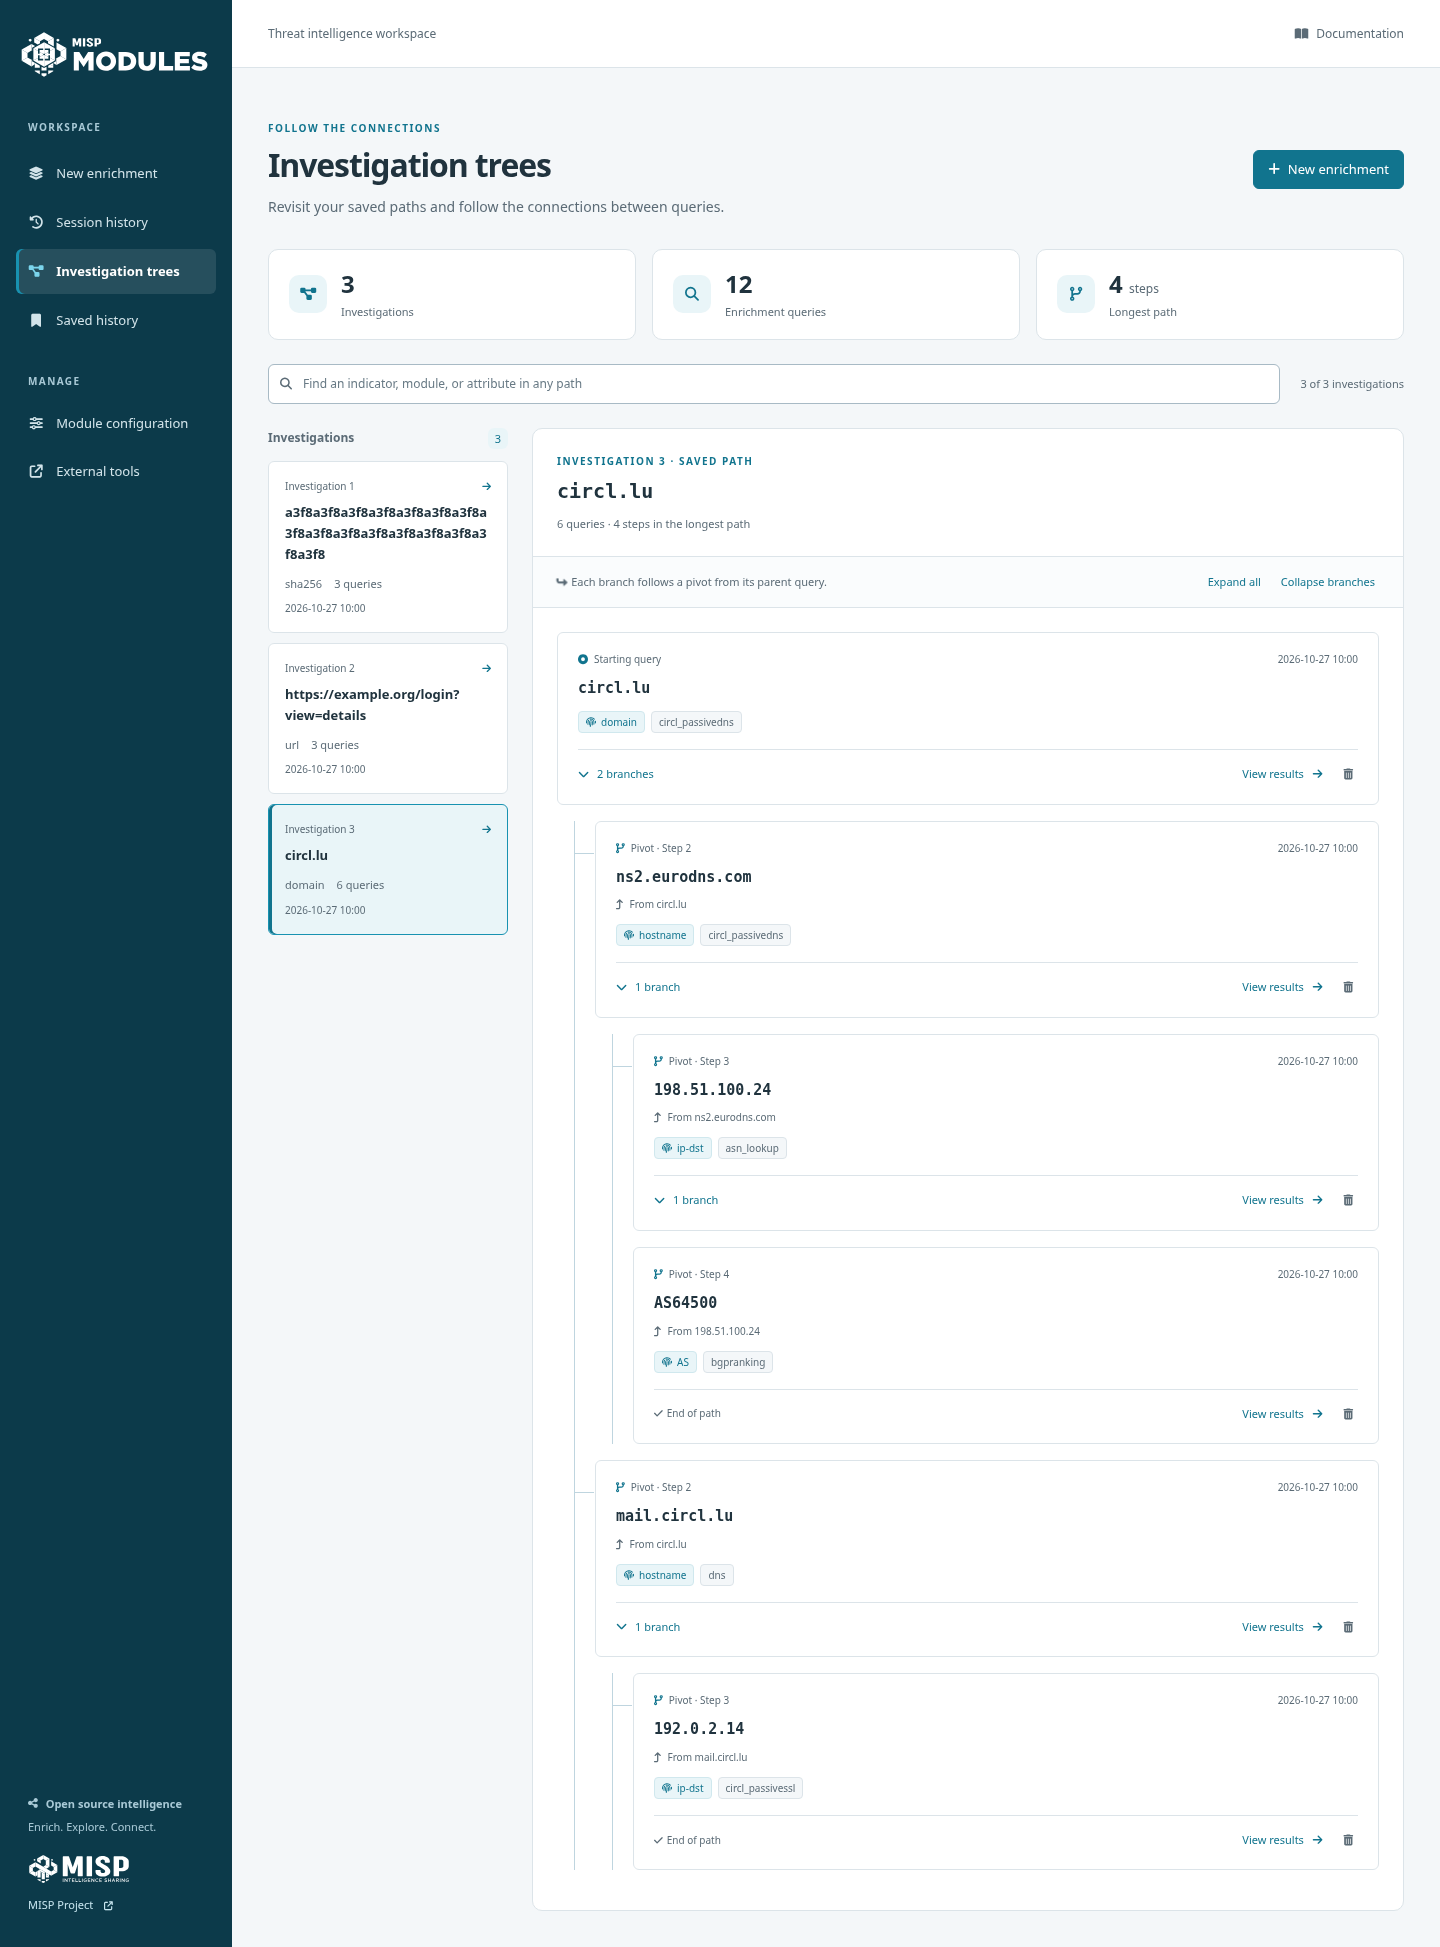
\includegraphics[width=\textwidth,height=.64\paperheight,keepaspectratio]{screenshots/current/investigations.png}
    \sources{Session history, saved trees and related-query paths in the current upstream interface.}
    \note{Follow parent and child queries, search paths, and keep context for pivots.
    The website can save session paths as investigation trees.
    For a website update, back up its database and apply shipped migrations with
    poetry run mmw db upgrade before restart. db init is for initial setup; db migrate
    generates a migration for developers, it does not apply shipped updates.
    The website and its production deployment were not exercised by the API-only lab.}
\end{frame}

\section{Develop and verify a module}

\begin{frame}{A small interface, a real contract}
    \begin{itemize}
        \item \code{introspection()}: supported input/output or import/export setup.
        \item \code{version()}: metadata, capabilities and configuration schema.
        \item \code{dict_handler(request=...)}: dictionary execution path supported
        by the current dispatcher.
        \item \code{handler(q=...)}: legacy JSON interface, still supported.
        \item Return useful \code{error} messages and valid result envelopes.
    \end{itemize}
    \begin{block}{Choose the result format deliberately}
        The lab's simple text module uses legacy results.
        For structured enrichment, start from a current \code{misp_standard}
        module and retain source UUIDs and references.
    \end{block}
    \note{The dispatcher tries dict\_handler first and falls back to handler.
    The supplied module implements both so their outputs can be compared.
    Avoid raising AttributeError accidentally within a dict\_handler; the current
    dispatcher's fallback also catches that exception.
    Do not copy the old deck's truncated DNS implementation with an except ellipsis.}
\end{frame}

\begin{frame}[fragile]{Metadata is part of discovery}
    \lstinputlisting[language=Python,firstline=5,lastline=13]{examples/custom/expansion/training_uppercase.py}
    \small
    \code{training_uppercase.py} gives the API identifier.
    The display name is \emph{Training uppercase}.
    \note{The module is a local-only contract demonstration.
    Use the filename as the API identifier and keep the display name descriptive.
    Returning metadata does not install dependencies or declare the module enabled
    for every organisation in MISP.}
\end{frame}

\begin{frame}[fragile]{A complete handler, with validation}
    \lstinputlisting[language=Python,firstline=24,lastline=36]{examples/custom/expansion/training_uppercase.py}
    \note{All lines are taken from the runnable file, not pseudocode.
    Show handler(q) below it in the source: it deserializes JSON and delegates here.
    The module is a contract demonstration, not a production enrichment source.
    It validates a nonempty text value and the prefix/config types before returning.
    Production modules also need bounded I/O and tests for dependency/provider failures.}
\end{frame}

\begin{frame}[fragile]{Load a local module without modifying the package}
\begin{lstlisting}
examples/custom/
  expansion/
    training_uppercase.py
\end{lstlisting}
\begin{lstlisting}[language=bash]
misp-modules -l 127.0.0.1 \
  --custom "$PWD/examples/custom"
\end{lstlisting}
    \begin{itemize}
        \item Pass the custom \emph{root}, not its \code{expansion} child.
        \item The loader discovers valid \code{.py} files; no \code{__all__} edit is needed.
        \item Restart, check logs and \code{/modules}, then enable/configure it in MISP.
    \end{itemize}
    \note{Run from this deck's directory. For the complete lab retain all README flags,
    including defaults and caching.
    Custom names must be unique: a custom module with the same identifier replaces
    an installed module. The service user needs read/traverse access.
    A non-editable pip installation uses an installed copy, so editing an unrelated
    checkout does not change a running service.}
\end{frame}

\begin{frame}{Test behavior across the service boundary}
    \begin{itemize}
        \item Compare dictionary and legacy handlers on valid and invalid input.
        \item Verify discovery and generated OpenAPI metadata.
        \item Check structured output and references using a local parser.
        \item Decode an export and verify indicator selection.
        \item Assert action status is \code{planned} in the dry run.
        \item Exercise defaults, API overrides, empty-value fallback,
        cache hits and error reporting.
    \end{itemize}
    \sources{The included \code{examples/verify_lab.py} performs 12 functional/contract tests.}
    \note{The tests fail if expected modules or startup options are absent.
    They do not contact external enrichment providers or perform a real publication.
    This scope does not validate MISP UI behavior, the website server, or vendor credentials.
    Direct handler tests alone cannot validate dispatcher caching or defaults.}
\end{frame}

\begin{frame}[fragile]{Workshop: discover, transform, verify}
    \begin{enumerate}
        \item \textbf{Discover}: find the lab modules and their formats in
        \code{/modules} and \code{/openapi.json}.
        \item \textbf{Transform}: parse a URL, decode a Zeek file and inspect
        an osquery publication plan.
        \item \textbf{Develop}: change the custom module's prefix and test a request
        override; inspect cache metrics and error responses.
    \end{enumerate}
\begin{lstlisting}[language=bash]
python3 examples/verify_lab.py \
  --url http://127.0.0.1:6666 -v
\end{lstlisting}
    \small
    Follow the README's full startup command before running the verifier.
    \note{Suggested timing: 10 minutes for discovery and structured enrichment,
    10 minutes for export/action interpretation, and 15--25 minutes for customization.
    Ask participants why a repeated UUID affects cache matching, why HTTP 200
    need not mean success, and why a planned pack is not an endpoint detection.
    The trainer guide includes expected answers and the limits of the lab.}
\end{frame}

\begin{frame}{What to take into the next integration}
    \begin{enumerate}
        \item Discover the \textbf{running} module set and its contracts.
        \item Separate service configuration, MISP enablement and provider readiness.
        \item Preserve evidence and review enrichment before operational use.
        \item Distinguish file generation, publication and activation.
        \item Test through the dispatcher when relying on its configuration or cache.
    \end{enumerate}
    \begin{block}{Keep the material current}
        Recheck the pinned source audit, exercise results and module-specific
        documentation before teaching a newer revision.
    \end{block}
    \note{Invite participants to propose a concrete integration and identify its family,
    input/output, source behavior, credentials, failure cases and validation plan.
    This replaces the old speculative roadmap with current, demonstrable capabilities.}
\end{frame}

\begin{frame}{References and next steps}
    \begin{itemize}
        \item \href{https://github.com/MISP/misp-modules}{MISP/misp-modules: code and current catalogue}
        \item \href{https://misp.github.io/misp-modules/}{Module documentation: install, contribute and module guides}
        \item \href{https://github.com/MISP/misp-modules/tree/main/website}{Standalone website and update instructions}
        \item \href{https://github.com/MISP/misp-modules-cli}{Standalone CLI client}
        \item This deck's \code{README.md}: pinned sources, trainer notes,
        reproducible lab and validation scope.
        \item Continue with \emph{Contributing MISP modules with an AI agent};
        see the companion \code{a.14-ai-assisted-misp-modules} deck.
    \end{itemize}
    \note{The README source audit uses immutable revision links for the reviewed behavior.
    The slide links deliberately lead to current project entry points.
    Use actual service discovery rather than treating a documentation catalogue as
    a guarantee that all modules are loaded or enabled.}
\end{frame}

\end{document}
